



\documentclass[first=dgreen,second=purple,logo=yellowexc]{aaltoslides}
%\documentclass{aaltoslides} % DEFAULT
%\documentclass[first=purple,second=lgreen,logo=redque,normaltitle,nofoot]{aaltoslides} % SOME OPTION EXAMPLES





% input encode
\usepackage[utf8]{inputenc}


%\usepackage[T1]{fontenc}
%\usepackage{lastpage}
%\usepackage{multirow}
%\usepackage{colortbl}
%\usepackage{comment}
%\usepackage{bm}
%\usepackage{natbib}


% Lipsum package generates bullshit
%\usepackage{lipsum}

% Set the document languages
%\usepackage[finnish,swedish,english]{babel}

% nomenclature
%\usepackage[intoc]{nomencl}

% math
\usepackage{amsmath}

% bibliograph
%\usepackage{natbib}

% For algorithms
\usepackage{algorithm}
\usepackage{algorithmic}

% math font
\usepackage{amsfonts}

% theory
%\usepackage{amsthm}

% double bracket
\usepackage{stmaryrd}

% special math symbol
\usepackage{amssymb}

% use enumerate environment
%\usepackage{enumitem}

% use \url \hyperref, make reference clickable
\usepackage{hyperref}

% use lastpage to inde
\usepackage{lastpage}



%-------------------
%
% set
%
%-------------------
\newcommand{\Acal}{\mathcal{A}}
\newcommand{\Bcal}{\mathcal{B}}
\newcommand{\Ccal}{\mathcal{C}}
\newcommand{\Dcal}{\mathcal{D}}
\newcommand{\Ecal}{\mathcal{E}}
\newcommand{\Fcal}{\mathcal{F}}
\newcommand{\Gcal}{\mathcal{G}}
\newcommand{\Hcal}{\mathcal{H}}
\newcommand{\Ical}{\mathcal{I}}
\newcommand{\Jcal}{\mathcal{J}}
\newcommand{\Kcal}{\mathcal{K}}
\newcommand{\Lcal}{\mathcal{L}}
\newcommand{\Mcal}{\mathcal{M}}
\newcommand{\Ncal}{\mathcal{N}}
\newcommand{\Ocal}{\mathcal{O}}
\newcommand{\Pcal}{\mathcal{P}}
\newcommand{\Qcal}{\mathcal{Q}}
\newcommand{\Rcal}{\mathcal{R}}
\newcommand{\Scal}{\mathcal{S}}
\newcommand{\Tcal}{\mathcal{T}}
\newcommand{\Ucal}{\mathcal{U}}
\newcommand{\Vcal}{\mathcal{V}}
\newcommand{\Wcal}{\mathcal{W}}
\newcommand{\Xcal}{\mathcal{X}}
\newcommand{\Ycal}{\mathcal{Y}}
\newcommand{\Zcal}{\mathcal{Z}}

\newcommand{\RR}{\mathbb{R}}
\newcommand{\ZZ}{\mathbb{Z}}

%-------------------
%
% vector
%
%-------------------
\newcommand{\va}{\mathbf {a}}
\newcommand{\vb}{\mathbf {b}}
\newcommand{\vc}{\mathbf {c}}
\newcommand{\vd}{\mathbf {d}}
\newcommand{\ve}{\mathbf {e}}
\newcommand{\vf}{\mathbf {f}}
\newcommand{\vg}{\mathbf {g}}
\newcommand{\vh}{\mathbf {h}}
\newcommand{\vi}{\mathbf {i}}
\newcommand{\vj}{\mathbf {j}}
\newcommand{\vk}{\mathbf {k}}
\newcommand{\vl}{\mathbf {l}}
\newcommand{\vm}{\mathbf {m}}
\newcommand{\vn}{\mathbf {n}}
\newcommand{\vo}{\mathbf {o}}
\newcommand{\vp}{\mathbf {p}}
\newcommand{\vq}{\mathbf {q}}
\newcommand{\vr}{\mathbf {r}}
\newcommand{\vs}{\mathbf {s}}
\newcommand{\vt}{\mathbf {t}}
\newcommand{\vu}{\mathbf {u}}
\newcommand{\vv}{\mathbf {v}}
\newcommand{\vw}{\mathbf {w}}
\newcommand{\vx}{\mathbf {x}}
\newcommand{\vy}{\mathbf {y}}
\newcommand{\vz}{\mathbf {z}}
\newcommand{\vmu}{\mathbf {\mu}}
\newcommand{\valpha}{\mathbf {\alpha}}
\newcommand{\vlambda}{\mathbf {\lambda}}
\newcommand{\vAlpha}{\mathbf {\Alpha}}
\newcommand{\vbeta}{\mathbf {\beta}}
\newcommand{\vBeta}{\mathbf {\Beta}}
\newcommand{\vgamma}{\mathbf {\gamma}}
\newcommand{\vGamma}{\mathbf {\Gamma}}
\newcommand{\vdelta}{\mathbf {\dalta}}
\newcommand{\vDelta}{\mathbf {\Dalta}}
\newcommand{\vone}{\mathbf {1}}
\newcommand{\vzero}{\mathbf {0}}
\newcommand{\vell}{\mathbf {\ell}}
\newcommand{\vxi}{\mathbf{\xi}}
\newcommand{\vphi}{\mathbf{\phi}}
\newcommand{\vPhi}{\mathbf{\Phi}}

%-------------------
%
% math operation
%
%-------------------
\newcommand{\argmax}{\textbf{argmax}}
\newcommand{\argmin}{\textbf{argmin}}
\newcommand{\sign}{\textbf{sign}}
\newcommand{\maximize}{\textbf{max}}
\newcommand{\minimize}{\textbf{min}}
\newcommand{\argkmax}{\textbf{argkmax}}
\newcommand{\argkmin}{\textbf{argkmin}}
\newcommand{\kmaximize}{\textbf{kmax}}
\newcommand{\kminimize}{\textbf{kmin}}
\newcommand{\st}{\textbf{s.t.}}
\newcommand{\set}[1]{\{ #1 \}}
%\newcommand{\ind}[1]{{\llbracket #1 \rrbracket}}
\newcommand{\ind}[1]{\mathbf{1}_{\{#1\}}}
\newcommand{\norm}[1]{\left|\left| #1 \right|\right|}
\newcommand{\ip}[2]{\langle #1, #2 \rangle}
\newcommand{\var}{\textbf{Var}}
\newcommand{\E}{\textbf{E}}
\newcommand{\exponential}[1]{e^{ #1 }}


\newcommand{\Gva}{G_{\va}}
%-------------------
%
% writings
%
%-------------------
\newcommand{\eqdef}{\overset{{\rm \mbox{\tiny def}}}{=}}
\newcommand{\sbf}[1]{\boldsymbol{#1}}
\newcommand{\mbf}[1]{\mathbf{#1}} 
\newcommand{\etal}{{\em et al.}}

\newcommand{\svmstruct}{{\sc ssvm}}
\newcommand{\mmmn}{{\sc m$^3$n}}
\newcommand{\svm}{{\sc svm}}
\newcommand{\mmcrf}{{\sc mmcrf}}
\newcommand{\smo}{{\sc smo}}
\newcommand{\crf}{{\sc crf}}
\newcommand{\nphard}{$\Ncal\Pcal$-hard}
\newcommand{\nphardness}{$\Ncal\Pcal$-hardness}
\newcommand{\iis}{{\sc iis}}
\newcommand{\memm}{{\sc memm}}
\newcommand{\lr}{{\sc lr}}
\newcommand{\svmlight}{{\sc svmlight}}
\newcommand{\libsvm}{{\sc libsvm}}
\newcommand{\svmcascade}{{\sc svmcascade}}
\newcommand{\adaboost}{{\sc adaboost}}
\newcommand{\adaboostmh}{{\sc adaboost.mh}}
\newcommand{\bagging}{{\sc bagging}}
\newcommand{\vrtree}{{\sc vr-tree}}
\newcommand{\deepboosting}{{\sc deepboosting}}
\newcommand{\loo}{{\sc loo}}
\newcommand{\mtl}{{\sc mtl}}
\newcommand{\sdp}{{\sc sdp}}
\newcommand{\iqp}{{\sc iqp}}
\newcommand{\qp}{{\sc qp}}
\newcommand{\daggraph}{{\sc dag}}
\newcommand{\lp}{{\sc lp}}

\newcommand{\hatf}{{\hat{f}}}
\newcommand{\p}{\sc p}
\newcommand{\n}{\sc n}
\newcommand{\pp}{\sc pp}
\newcommand{\pn}{\sc pn}
\newcommand{\nn}{\sc nn}
\newcommand{\maxcut}{{\sc max-cut}}
\newcommand{\greedy}{{\sc greedy}}
\newcommand{\kernelcascade}{{\sc kernel cascade}}
\newcommand{\netrate}{{\sc netrate}}
\newcommand{\netinf}{{\sc netinf}}
\newcommand{\spin}{{\sc spin}}
\newcommand{\vI}{\mathbf{I}}
\newcommand{\tp}{^{\intercal}}
\newcommand{\mve}{{\sc mve}}
\newcommand{\amm}{{\sc amm}}
\newcommand{\mam}{{\sc mam}}
\newcommand{\rta}{{\sc rta}}
\newcommand{\lasso}{{\sc lasso}}
\newcommand{\mle}{{\sc mle}}
\newcommand{\map}{{\sc map}}
\newcommand{\rbf}{{\sc rbf}}
\newcommand{\mlknn}{{\sc ml-knn}}
\newcommand{\knn}{{\sc knn}}
\newcommand{\iblr}{{\sc iblr}}
\newcommand{\cc}{{\sc cc}}
\newcommand{\pcc}{{\sc pcc}}
\newcommand{\ecc}{{\sc ecc}}
\newcommand{\br}{{\sc br}}
\newcommand{\corrlog}{{\sc corrlog}}
\newcommand{\ilgs}{{\sc ilgs}}
\newcommand{\ilrs}{{\sc ilrs}}
\newcommand{\cpp}{{\sc c}}
\newcommand{\matlab}{{\sc matlab}}
\newcommand{\openmp}{{\sc openmp}}
\newcommand{\python}{{\sc python}}
\newcommand{\cvx}{{\sc cvx}}
\newcommand{\lda}{{\sc lda}}
\newcommand{\kkt}{{\sc k.k.t}}
\newcommand{\lbp}{{\sc lbp}}
\newcommand{\anova}{{\sc anova}}

\renewcommand{\algorithmicrequire}{\textbf{Input:}}
\renewcommand{\algorithmicensure}{\textbf{Output:}}



\newcommand{\Upsilonb}{\pmb \Upsilon}
\newcommand{\phib}{\pmb \phi}
\newcommand{\psib}{\pmb \psi}
\newcommand{\varphib}{\pmb \varphi}
\newcommand{\phibh}{\hat\phib}
\newcommand{\psibh}{\hat \psib}
\newcommand{\vYcal}{\pmb \Ycal}
\newcommand{\vXcal}{\pmb \Xcal}
\newcommand{\vFcal}{\pmb \Fcal}
%-------------------
%
% others
%
%-------------------




%\newtheorem{definition}{Definition}
%\newtheorem{theory}{Theory}
%\newtheorem{lemma}{Lemma}

















\title{Structured output prediction for multilabel classification}
\author{Hongyu Su}



\institute[ICS]{
Helsinki Institute for Information Technology HIIT\\
Department of Computer Science, Aalto University
}

\aaltofootertext{Structured output prediction}{\today}{\arabic{page}\ }


\date{ \today} %\date{Version 1.0, \today}

\iffalse
\AtBeginSection[]
{
  \begin{frame}<beamer>{Outline}
    \tableofcontents[currentsection,subsection]
  \end{frame}
}
\fi




%--------------------------------
%
% document
%
%--------------------------------

\begin{document}

\aaltotitleframe
\footnotesize

%
\begin{frame}{Multilabel classification}
	\begin{itemize}\footnotesize
		\item {\em Multilabel classification} is an important research field in machine learning.
		\item Input variable $\vx\in\vXcal$ is in $d$ dimensional input space $\vXcal=\RR^d$.
		\item Output variable $\vy=(y_1,\cdots,y_l)\in\vYcal$ is a binary vector consist of $l$ binary variables $y_j\in\{+1,-1\}$.
		\item $\vy$ is called a multilabel, $y_j$ is called a microlabel.
		\item Output space is composed by a Cartesian product of $l$ sets
		\begin{align*}
			\vYcal=\Ycal_1\times\cdots\times\Ycal_l,\,\Ycal_i=\{+1,-1\}.
		\end{align*}
		\item For example, in document classification, a document $\vx$ can be classified as ``news'', ``movie'', and ``science''
		\begin{align*}
\vy=(\underbrace{+1}_{\text{news}},\underbrace{+1}_{\text{movie}},\underbrace{-1}_{\text{sports}},\underbrace{-1}_{\text{politics}},\underbrace{-1}_{\text{finance}},\underbrace{+1}_{\text{science}},\underbrace{-1}_{\text{art}}).
		\end{align*}\footnotesize
		\item The goal is to find a mapping function $f\in\Hcal$ that predicts the best values of an output given an input $f:\vXcal\rightarrow\vYcal$.
	\end{itemize}
\end{frame}

%
\begin{frame}{Central problems in multilabel classification}
	\begin{itemize}\footnotesize
		\item The size of the output space (searching space) is exponential in the number of microlabels.
		\begin{align*}
			\vYcal=\Ycal_1\times\cdots\times\Ycal_l,\,\Ycal_i=\{+1,-1\}\quad|\vYcal| = 2^l.
		\end{align*}
		\item The dependency of microlabels needs to be exploited to improve the prediction performance.
		\begin{itemize}\footnotesize
			\item If a document is about ``movie'', then it is more likely to be about ``art'' than ``science''.
		\end{itemize}
	\end{itemize}
\end{frame}

%
\begin{frame}{Real world applications}
	\begin{itemize}\footnotesize
		\item Social network, information can spread through multiple users. 
		\begin{tabular}{p{3cm}p{10cm}} 
	    \multirow{2}{*}{
\includegraphics[scale = 0.06]{./figures/facebookvideo.png}} & \\
		& $\vy=(\underbrace{+1}_{\text{Ted}},\underbrace{-1}_{\text{Alice}},\underbrace{+1}_{\text{David}},\underbrace{-1}_{\text{Mark}},\underbrace{+1}_{\text{Alex}},\underbrace{-1}_{\text{Zoe}},\underbrace{-1}_{\text{Frank}})$\\
	    \end{tabular}
		\item Image annotation, an image can associate with multiple tags.
		\begin{tabular}{p{3cm}p{10cm}}
        \multirow{2}{*}{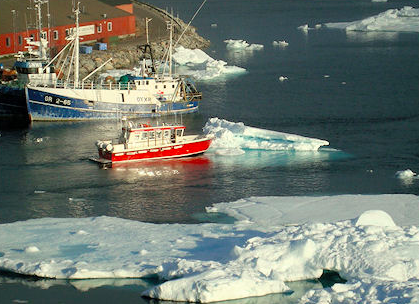
\includegraphics[scale = 0.11]{./figures/boatsea.png}} & \\
		& $\vy=(\underbrace{+1}_{\text{boat}},\underbrace{+1}_{\text{sea}},\underbrace{-1}_{\text{sun}},\underbrace{-1}_{\text{beach}},\underbrace{-1}_{\text{people}},\underbrace{+1}_{\text{ice}},\underbrace{+1}_{\text{land}})$\\
        \end{tabular}
		\item Document classification, an article can be assigned to multiple categories.
		\begin{tabular}{p{3cm}p{10cm}} 
        \multirow{2}{*}{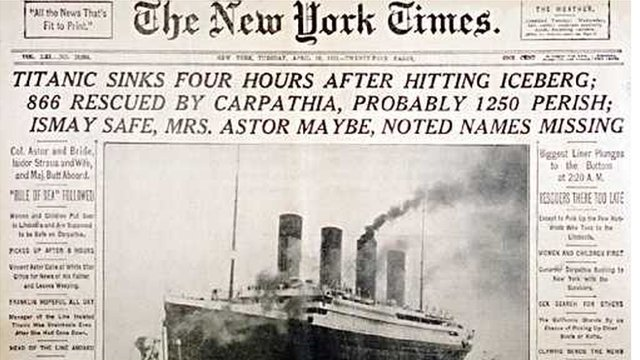
\includegraphics[scale = 0.11]{./figures/titanic.jpg}} & \\
		& $\vy=(\underbrace{+1}_{\text{news}},\underbrace{+1}_{\text{economics}},\underbrace{-1}_{\text{sports}},\underbrace{-1}_{\text{politics}},\underbrace{-1}_{\text{movie}},\underbrace{-1}_{\text{science}},\underbrace{-1}_{\text{art}})$\\
        \end{tabular}
		\item Drug discovery, a drug can be effective for multiple symptoms.
		\begin{tabular}{p{3cm}p{10cm}} 
        \multirow{2}{*}{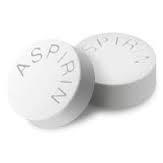
\includegraphics[scale = 0.25]{./figures/aspirin.jpg}} & \\
		& $\vy=(\underbrace{+1}_{\text{heart}},\underbrace{+1}_{\text{stroke}},\underbrace{+1}_{\text{blood}},\underbrace{+1}_{\text{fever}},\underbrace{-1}_{\text{digest}},\underbrace{-1}_{\text{liver}},\underbrace{+1}_{\text{swelling}})$\\
        \end{tabular}
	\end{itemize}
\end{frame}

%
\begin{frame}{Flat multilabel classification approaches}
	\begin{itemize}\footnotesize
		\item The categorization is proposed in \cite{Tsoumakas10mining}
		\item Problem transformation
		\begin{itemize}\footnotesize
			\item Model the multilabel classification as a collection of single-label classification problems and solve each problem independently.
			\item For example, \mlknn\ \cite{Zhang07mlknn}, \cc\ \cite{Read09classifier,Read11classifier}, \iblr\ \cite{Cheng09combining}.
		\end{itemize}
		\item Algorithm adaptation 
		\begin{itemize}\footnotesize
			\item Modify the single-label classification algorithm for multilabel classification problems.
			\item For example, \adaboostmh\ \cite{Schapire99improved,Esuli2008boosting}, \corrlog\ \cite{Bian12corrlog}, \mtl\ \cite{Argyriou08convex}.
		\end{itemize}
		\item These approaches does not model the dependency structure explicitly.
	\end{itemize}
\end{frame}

%
\begin{frame}{Structured output prediction}
	\begin{itemize}\footnotesize
		\item Model the dependency structure with an output graph defined on microlabels.
		\item The categorization is proposed in \cite{Su2014Multilabel}.
		\item Hierarchical classification
		\begin{itemize}\footnotesize
			\item The output graph is a rooted tree or a \daggraph\ defining different levels of granularities.
			\item For example, \svmstruct\ \cite{THJA04,TJTA05}.
		\end{itemize}
		\item Graph labeling
		\begin{itemize}\footnotesize
			\item The output graph takes a more general form (e.g., a tree, a chain).
			\item For example, \crf\ \cite{lafferty01,taskar02}, \mmmn\ \cite{Taskar04max}, \mmcrf\ \cite{Rousu07, su10structured}, \spin\ \cite{su14structured}.
		\end{itemize}
		\item These approaches assume the output graph is known {\em apriori}.
	\end{itemize}
\end{frame}

%
\begin{frame}{Contributions}
	\begin{itemize}\footnotesize
		\item Structured output prediction models when the output graph is known.
		\begin{itemize}\footnotesize
			\item \spin\ for network influence prediction \cite{su14structured}.
			\item \mmcrf\ to work with general output graph structures \cite{su10structured}.
		\end{itemize}
		\item Structured output prediction models working with unknown output graph.
		\begin{itemize}\footnotesize
			\item \mve\ to combine multiple structured output predictors with ensemble \cite{su11mutitask}.
			\item \amm\ and \mam\ to aggregate the inference results from multiple structured output predictors \cite{su2013multilabelacml,su15multilabel}.
			\item \rta\ to perform joint learning and inference over a collection of random spanning trees \cite{su14multilabelnips}.
		\end{itemize}
		\item Codes for developed models are available from \href{http://hongyusu.github.io}{http://hongyusu.github.io}.
	\end{itemize}
\end{frame}


%
\begin{frame}{Outline}
\end{frame}

%
\begin{frame}{Preliminaries}
	\begin{itemize}\footnotesize
		\item Training examples come in pairs $(\vx,\vy)\in\vXcal\times\vYcal$.
		\item $\vx\in\vXcal$ is an arbitrary input space.
		\item $\vYcal$ is an output space of a collection of $\ell$-dimensional {\em multilabels}.
		\begin{align*}\footnotesize
			\vy=(y_1,\cdots,y_{\ell})\in\vYcal.
		\end{align*}
		\item $y_i$ is a {\em microlabel} and $y_i\in\{1,\cdots,r_i\}, r_i\in\ZZ$.
		\item For example, multilabel binary classification $y_i\in\{-1,+1\}$.
		\item We are given a set of $m$ training examples $\{(\vx_i,\vy_i)\}_{i=1}^m$.
		%\item An arbitrary pair $(\vx_i,\vy),\,\vy_\in\vYcal$ is called pseudo-example.
		\item Each example $(\vx,\vy)$ is mapped into a joint feature space $\phib(\vx,\vy)$.
		\item $\vw$ is the weight vector in the joint feature space.
		\item Define a linear score function $F(\vw,\vx,\vy) = \ip{\vw}{\phib(\vx,\vy)}$.
		\item $\vw$ makes sure example $\vx$ with correct multilabel $\vy$ achieves higher score than with any other incorrect multilabel $\vy'\in\vYcal$.
	\end{itemize}
\end{frame}

\begin{frame}{Inference problem}
	\begin{itemize}
		\item The prediction $\vy_{\vw}(\vx)$ of an input $\vx$ is the multilabel $\vy$ that maximizes the score function 
		\begin{align}\footnotesize
			\vy_{\vw}(\vx) = \underset{\vy\in\vYcal}{\argmax}\,\ip{\vw}{\phib(\vx,\vy)}. \label{inference}
		\end{align}
		\item Search space $|\vYcal|=2^{\ell}$ is exponential in size.
		\item (\ref{inference}) is called {\em inference} problem which is \nphard\ for most output feature maps.
		\item We aim at using an output feature map in which the inference can be solved with a polynomial algorithm, e.g., dynamic programming.
	\end{itemize}
\end{frame}

%
\begin{frame}{Input-output feature maps}
	\begin{itemize}\footnotesize
		\item We assume that the joint feature map $\phib$ is a potential function on a Markov network $G=(E,V)$.
		\item A vertex $v_i\in V$ corresponds to a microlabel $y_i$, an edge $(v_i,v_j)\in E$ corresponds to the pairwise correlation of the microlabel $y_i$ and $y_j$.
		\item $G$ models potential pairwise correlations.
		\begin{center}
			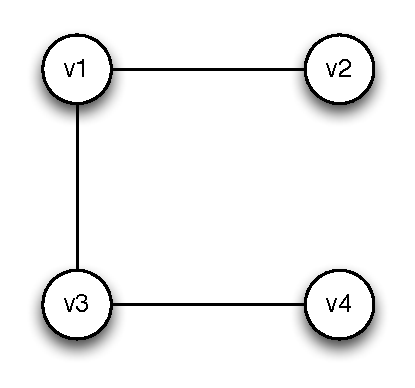
\includegraphics[scale=0.3]{./figures/outputgraph.pdf}
		\end{center}
		\item $\varphib(\vx)\in\RR^d$ is the input feature map, e.g., bag-of-words of a document.
		\item $\psib(\vy)\in\RR^{4|E|}$ is the output feature map which maps the multilabel $\vy$ into a collection of edges and labels
		\begin{align*}\footnotesize
			\varphib(\vy) = (u_{e})_{e\in E},u_e\in\{-1,+1\}^2.
		\end{align*}
	\end{itemize}
\end{frame}

%
\begin{frame}{An example of output feature map}
	\begin{itemize}\footnotesize
		\item Markov network $G=(E,V)$
		\begin{center}
			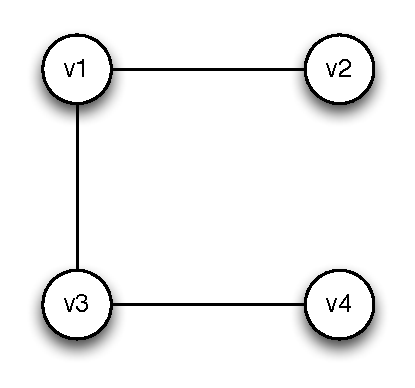
\includegraphics[scale=0.3]{./figures/outputgraph.pdf}
		\end{center}
		\item Multilabel $\vy$
		\begin{align*}
			\vy&=(y_1,y_2,y_3,y_4)=(+1,-1,+1,+1)
		\end{align*}
		\item Output feature map $\psib(\vy)$
		\begin{align*}
			\psib(\vy) &= ( \underbrace{\underbrace{0}_{--}, \underbrace{0}_{-+}, \underbrace{1}_{+-}, \underbrace{0}_{++},}_{(v_1,v_3)} 
			\underbrace{\underbrace{0}_{--}, \underbrace{0}_{-+}, \underbrace{0}_{+-}, \underbrace{1}_{++},}_{(v_1,v_2)}
			\underbrace{\underbrace{0}_{--}, \underbrace{0}_{-+}, \underbrace{0}_{+-}, \underbrace{1}_{++}}_{(v_3,v_4)})
		\end{align*}
	\end{itemize}
\end{frame}

%
\begin{frame}{Joint feature map}
	\begin{itemize}\footnotesize
		\item The joint feature is the Kronecker product of $\varphib(\vx)$ and $\psib(\vy)$
		\begin{align*}\footnotesize
			\phib(\vx,\vy) = (\phib_e(\vx,\vy))_{e\in E}=(\varphib(\vx)\otimes\psib_e(\vy_e))_{e\in E}.
		\end{align*}
		\begin{center}
			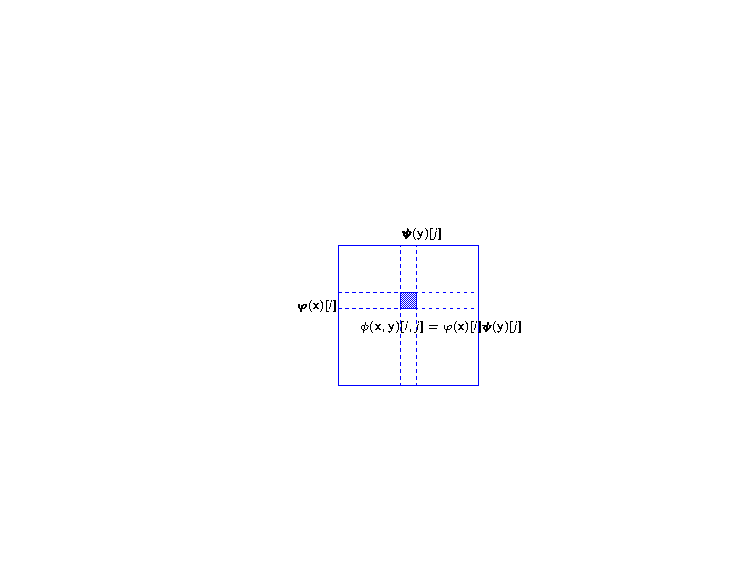
\includegraphics[scale = 1]{./figures/tensor_label.pdf}
		\end{center}
		\item The score function can be factorized by the output graph $G$
		\begin{align*}
			F(\vw,\vx,\vy) = \ip{\vw}{\phib(\vx,\vy)} = \sum_{e\in E}\ip{\vw_e}{\phib_e(\vx,\vy_e)}.
		\end{align*}
	\end{itemize}
\end{frame}

%
\begin{frame}{Primal optimization problem}
	\begin{itemize}\footnotesize
		\item To learn parameter $\vw$, we aim to maximize the magin between correct pair $(\vx_i,\vy_i)$ and all the other incorrect pairs $(\vx_i,\vy),\vy/in/vYcal\/vy_i$.
		\item The primal optimization problem is defined as \cite{Rousu07, su10structured}
		\begin{align*}
			\underset{\vw,\xi_k}{\minimize} & \quad \frac{1}{2}\norm{\vw}^2 + C\sum_{k=1}^{m}\xi_k\\
			\st & \quad \ip{\vw}{\phib(\vx_k,\vy_k)} - \ip{\vw}{\phib(\vx_k,\vy)}  \geq \ell(\vy_k,\vy) -  \xi_k, \\
			& \quad \xi_k\ge0\, , \forall\ \vy\in\vYcal, k \in \set{1,\dots,m}.
		\end{align*}
	\end{itemize}
\end{frame}

%
\begin{frame}{}
	\begin{itemize}\footnotesize
		\item
	\end{itemize}
\end{frame}

%
\begin{frame}{}
	\begin{itemize}\footnotesize
		\item
	\end{itemize}
\end{frame}

%
\begin{frame}{}
	\begin{itemize}\footnotesize
		\item
	\end{itemize}
\end{frame}

%
\begin{frame}{}
	\begin{itemize}\footnotesize
		\item
	\end{itemize}
\end{frame}

%
\begin{frame}{}
	\begin{itemize}\footnotesize
		\item
	\end{itemize}
\end{frame}

%
\begin{frame}{}
	\begin{itemize}\footnotesize
		\item
	\end{itemize}
\end{frame}

%
\begin{frame}{Structured output learning}
	\begin{itemize}\footnotesize
		\item There is an \textit{output graph} connecting multiple labels.
		\begin{itemize}\footnotesize
			\item A set of nodes represents multiple labels.
			\item A set of edges represents the correlation between labels.
		\end{itemize}
		\item Hierarchical classification:
		\begin{itemize}\footnotesize
			\item The output graph is a rooted tree or a directed graph defining different levels of granularities.
			\item For example, \svmstruct, ...
		\end{itemize}
		\item Graph labeling:
		\begin{itemize}\footnotesize
			\item The output graph often takes a general form (e.g., a tree, a chain).
			\item For example, \mmmn, \crf, \mmcrf, ...
		\end{itemize}
		\item The output graph is assumed to be known \textit{apriori}.
	\end{itemize}
\end{frame}



%
\begin{frame}{Research question}
	\begin{itemize}\footnotesize
		\item The output graph is hidden in many applications.
		\begin{itemize}\footnotesize
			\item For example, a surveillance photo can be tagged with ``building'', ``road'', ``pedestrian'', and ``vehicle''.
		\end{itemize}
		\item We study the problem in structured output learning when the output graph is not observed.
		\item In particular:
		\begin{itemize}\footnotesize
			\item Assume the dependency can be expressed by a complete set of pairwise correlations.
			\item Build a structured output learning model with a complete graph as the output graph.
			\item Solve the optimization problem and the inference problem (\nphard).
		\end{itemize}
	\end{itemize}
\end{frame}



%
\begin{frame}{Today}
	\begin{itemize}\footnotesize
		\item A structured prediction model which performs max-margin learning on a random sample of spanning tree.
		\item Two ways to combine the set of random spanning trees
		\begin{itemize}\footnotesize
			\item conical combination in NIPS paper.
			\item convex combination as future work.
		\end{itemize}
		\item Derivations and the corresponding optimization problems.
	\end{itemize}
\end{frame}



%
\begin{frame}[allowframebreaks]{Model}
	\begin{itemize}\footnotesize
		\item Training examples comes in pair $S=\{(\vx_i,\vy_i)\}_{i=1}^{m}\in\vXcal\times\vYcal$.
		\item A complete graph $G=(E,V)$ is used as the output graph.
		\item $\varphi(\vx)$ is the input feature map, e.g., a feature vector of $d$ dimension.
		\item $\Gamma_G(\vy)$ is the output feature map of $\vy$ on $G$ of $4\times |E|$ dimension
		\begin{align*}
			\Gamma_G(\vy) &= \{\Gamma_e(\vy_{e})\}_{e\in G},\\
			 \Gamma_e(\vy_{e}) &= [\vone_{\vy_{e}==00},\vone_{\vy_{e}==01},\vone_{\vy_{e}==10},\vone_{\vy_{e}==11}]
		\end{align*}
		\item A joint feature map of $(\vx_i,\vy_i)$
		\begin{align*}
			\phi_G(\vx_i,\vy_i) = \varphi(\vx_i)\otimes\Gamma_G(\vy_i) = \{\phi_e(x_i,\vy_{i,e})\}_{e\in G}.
		\end{align*}
		\item A compatibility score is defined as
		\begin{align*}
			F(\vx,\vy;\vw_G) = \ip{\vw_G}{\phi_G(\vx,\vy)}=\sum_{e\in G}\ip{\vw_{G,e}}{\phi_e(\vx,\vy_{e})}
		\end{align*}
		\item $\vw$ ensures an input $\vx_i$ with a correct multilabel $\vy_i$ achieves a higher score than with any incorrect multilabel $\vy\in\Ycal$.
		\item The predicted output $\vy(\vx)$ for a given input $\vx$ is computed by
		\begin{align*}
			\vy(\vx) = \underset{\vy\in\vYcal}{\argmax}\,F(\vx,\vy;\vw_G) = \underset{\vy\in\vYcal}{\argmax}\,\sum_{e\in G}\ip{\vw_{G,e}}{\phi_{G,e}(\vx,\vy_e)},
		\end{align*}
		which is called \textit{inference problem}.
		\item The {inference problem} is \nphard\ for most joint feature maps on the complete graph.
	\end{itemize}
\end{frame}



%
\begin{frame}{How to learn $\vw$ on a complete graph?}
	\begin{itemize}\footnotesize
		\item The \textit{margin} of an example $\vx_i$ is
		\begin{align*}
			\gamma_G(\vx_i;\vw_G) = F(\vx_i,{\color{aaltored} \vy_i};\vw_G) - \underset{{\color{aaltoblue}\vy\in\vYcal/\vy_i}}{\maximize}\,F(\vx_i,{\color{aaltoblue}\vy};\vw_G).
		\end{align*}
		\item $\vw$ is solved by \textit{max-margin principle} which aims to maximize $\gamma(\vx_i;\vw_G)$ over all training example $\vx_i,i\in\{1,\cdots,m\}$.
		\item The inference problem on a complete graph is \nphardness.
		\item The parameter space is quadratic in the number of microlabels $k$.
		\item We aim to use a joint feature map that allows the inference problem be solved in polynomial time.
	\end{itemize}
\end{frame}



%
\begin{frame}{Superposition of random trees}
	\begin{itemize}\footnotesize
		\item $S(G)$ is a complete set of spanning tree generate from $G$, $|S(G)| = \ell^{\ell-2}$.
		\item Recall $\phi_G(\vx,\vy) = \{\phi_{G,e}(\vx,\vy_e)\}_{e\in G},\vw_G = \{\vw_{G,e}\}_{e\in G},||\phi_G(\vx,\vy)||=||\vw_{G}||=1$.
		\item $\phi_T(\vx,\vy)=\{\phi_e(\vx,\vy)\}_{e\in T}$ is the projection of $\phi_G(\vx,\vy)$ on $T\in S(G)$.
		\item $\vw_{T}=\{\vw_{G,e}\}_{e\in T}$ is the projection of $\vw_G$ on $T\in S(G)$.
		\item Rewrite
		\begin{align*}
			F(\vx,\vy,\vw_G) &= \sum_{e\in G}\ip{\vw_{G,e}}{\phi_{G,e}(\vx,\vy_e)} \\
			& = \frac{1}{\ell^{\ell-2}}\sum_{T\in S(G)}\sqrt{\frac{\ell}{2}}\ip{\vw_{T}}{\phi_{T}(\vx,\vy_e)}\\
			& {\color{aaltored} =} \frac{1}{n}\sum_{i = 1}^{n}a_{T_i}\ip{\hat{\vw}_{T_i}}{\hat{\phi}_{T_i}(\vx,\vy_e)},\\
			||\hat{\phi}_T(\vx,\vy)||=||\hat{\vw}_{T}||=1,\, & \frac{1}{n}\sum_{i = 1}^{n}a_{T_i}^2=1, \, \frac{1}{n}\sum_{i = 1}^{n}a_{T_i}\le1,\, a_{T_i}\ge0,\, n=\ell^{\ell-2}.
		\end{align*}
	\end{itemize}
\end{frame}


%
\begin{frame}{How many trees?}
	\begin{itemize}\footnotesize
		\item If there is a predictor $\vw_G$ on complete graph achieves a margin on some training data, with high probability we need $n$ spanning tree predictors $\{\vw_{T_i}\}_{i=1}^n$ to achieve a close margin. $n$ is quadratic in terms of $\ell$.
		\item Recall
		\begin{align*}
			F(\vx,\vy,\vw_{\Tcal}) &= \frac{1}{n}\sum_{i = 1}^{n}a_{T_i}\underbrace{\ip{\hat{\vw}_{T_i}}{\hat{\phi}_{T_i}(\vx,\vy_e)}}_{F(\vx,\vy,\vw_{T_i})},\\
			||\hat{\phi}_T(\vx,\vy)||=||\hat{\vw}_{T}||=1,\, & \frac{1}{n}\sum_{i = 1}^{n}a_{T_i}^2=1, \, \frac{1}{n}\sum_{i = 1}^{n}a_{T_i}\le1,\, a_{T_i}\ge0,\, \xcancel{n=\ell^{\ell-2}}.
		\end{align*}
	\end{itemize}
\end{frame}


%
\begin{frame}[allowframebreaks]{Conical combination}
	\begin{itemize}\footnotesize
		\item A sample $\Tcal=\{T_1,\cdots,T_n\}$ of $n$ spanning trees drawn from $G$.
		\item Normalized feature vectors $\hat{\phi}_{T_i}(\vx,\vy)=\frac{\phi_{T_i}(\vx,\vy)}{||\phi_{T_i}(\vx,\vy)||}, \, T_i\in\Tcal$.
		\item Normalized feature weights $\hat{\vw}_{T_i}=\frac{\vw_{T_i}}{||\vw_{T_i}||}, \, T_i\in\Tcal$.
		\item Conical combination of spanning trees
		\begin{align*}
			F(\vx,\vy,\vw_{\Tcal}) &= \frac{1}{\sqrt{n}}\sum_{i=1}^{n}q_i\underbrace{\ip{\hat{\vw}_{T_i}}{\hat{\phi}_{T_i}(\vx,\vy)}}_{F(\vx,\vy,\vw_{T_i})}\\
			\sum_{i=1}^{n}q_i^2 &= 1,\, q_i \ge 0,\, \forall i\in\{1,\cdots,n\}.
		\end{align*}
		\item To solve $\{\vw_{T_i}\}_{T_i\in\Tcal}$, we need to work on the optimization problem
		\begin{align*}
			\underset{\vxi,\gamma,\vq,\Wcal}{\minimize} \quad& \frac{1}{2\gamma^2} + \frac{C}{\gamma}\sum_{k=1}^m\xi_k\\
			\st \quad& \frac{1}{\sqrt{n}}\sum_{i=1}^{n}q_i\ip{\hat{\vw}_{T_i}}{\hat{\phi}_{T_i}(\vx_k,\vy_k)} -\underset{\vy\in\vYcal}{\maximize}\frac{1}{\sqrt{n}}\sum_{i=1}^{n}q_i\ip{\hat{\vw}_{T_i}}{\hat{\phi}_{T_i}(\vx_k,\vy)}\\
			&\ge \gamma-\xi_k, \xi_k\ge 0,\forall k\in\{1,\cdots,m\},\sum_{i=1}^nq_i^2=1,q_i\ge0,\forall i\in\{1,\cdots,n\}.
		\end{align*}
		\item This is equivalent to
		\begin{align*}
			\underset{\vw_{T_i},\xi_i}{\minimize} & \quad \frac{1}{2}\sum_{i=1}^{n}\norm{\vw_{T_i}}^2 + C\sum_{k=1}^{m}\xi_k\\
			\st & \quad \frac{1}{\sqrt{n}}\sum_{i=1}^{n}{ \langle \vw_{T_i}, \phib_{T_t}(\vx_k,\vy_k) \rangle} - \underset{\vy \neq \vy_k}{\maximize\ } \frac{1}{\sqrt{n}}\sum_{i=1}^{n}{\langle \vw_{T_t}, \phib_{T_i}(\vx_k,\vy) \rangle } \geq 1 -  \xi_k, \\
			& \quad \xi_k\ge0\, , \forall\ k \in \set{1,\dots,m}.
		\end{align*}
	\end{itemize}
\end{frame}


\begin{frame}{Inference Problem}
	\begin{itemize}
		\item The inference problem of \rta\ is defined as finding the multilabel $\vy_{\Tcal}(\vx)$ that maximizes the sum of scores over a collection of trees
		\begin{align*}
			\vy_{\Tcal}(\vx) = \underset{\vy\in\vYcal}{\argmax}\,{\color{aaltoblue}F_{\Tcal}(\vx,\vy;\vw_{\Tcal})} = \underset{\vy\in\vYcal}{\argmax}\,\sum_{t=1}^{n}\ip{\vw_{T_t}}{\phi_{T_t}(\vx,\vy)}.
		\end{align*}
		\item The inference problem on each individual spanning tree can be solve efficiently in $\Theta(l)$ by \textit{dynamic programming}
		\begin{align*}
			\vy_{T_t}(\vx) = \underset{\vy\in\vYcal}{\argmax}\,{\color{aaltored}F_{T_t}(\vx,\vy;\vw_{T_t})}= \underset{\vy\in\vYcal}{\argmax}\,\ip{\vw_{T_t}}{\phi_{T_t}(\vx,\vy)}.
		\end{align*}
		\item There is no guarantee that there exists a tree $T_t\in\Tcal$ in which the maximizer of ${\color{aaltored}F_{T_t}}$ is the maximizer of ${\color{aaltoblue}F_{\Tcal}}$.
	\end{itemize}
\end{frame}




%
\begin{frame}[allowframebreaks]{Fast Inference Over a Collection of Trees}
	\begin{itemize}
		\item For each tree $T_t$, instead of computing the best multilabel $\vy_{T_t}$, we compute $K$-best multilabels in $\Theta(Kl)$ time
		\begin{align*}
			\Ycal_{T_t,K} = \{\vy_{T_t,1},\cdots,\vy_{T_t,K}\}.
		\end{align*}
		\item Performing the same computation on all trees gives a candidate list of $n\times K$ multilabels in $\Theta(nKl)$ time
		\begin{align*}
			\Ycal_{\Tcal,K}=\Ycal_{T_1,K}\cup\cdots\Ycal_{T_n,K}.
		\end{align*}
		\item For now, we assume the best scoring multilabel of a collection of trees exists in the list $\Ycal_{\Tcal,K}$. 
		\item We proved that with a high probability $\vy_{\Tcal}$ will appear in $\Ycal_{\Tcal,K}$.
		\item We can identify $\vy_{\Tcal}$ from $\Ycal_{\Tcal,K}$.
	\end{itemize}
\end{frame}


%
\begin{frame}[allowframebreaks]{Convex combination}
	\begin{itemize}\footnotesize
		\item A sample $\Tcal$ of $n$ spanning trees drawn from $G$.
		\item Normalized feature weights $\hat{\vw}_{T_i}=\frac{\vw_{T_i}}{||\vw_{T_i}||}, \, T_i\in\Tcal$.
		\item Normalized feature vectors $\hat{\phi}_{T_i}(\vx,\vy)=\frac{\phi_{T_i}(\vx,\vy)}{||\phi_{T_i}(\vx,\vy)||}, \, T_i\in\Tcal$.
		\item Convex combination of spanning trees
		\begin{align*}
			F(\vx,\vy,\vw_{\Tcal}) &= \frac{1}{{n}}\sum_{i=1}^{n}q_i\ip{\hat{\vw}_{T_i}}{\hat{\phi}_{T_i}(\vx,\vy)}\\
			\sum_{i=1}^{n}q_i &= 1,\, q_i \ge 0,\, \forall i\in\{1,\cdots,n\}.
		\end{align*}
		\item To solve $\{\vw_{T_i}\}_{T_i\in\Tcal}$, we need to work on the optimization problem
		\begin{align*}
			\underset{\vxi,\gamma,\vq,\Wcal}{\minimize} \quad& \frac{1}{2\gamma^2} + \frac{C}{\gamma}\sum_{k=1}^m\xi_k\\
			\st \quad& \frac{1}{{n}}\sum_{i=1}^{n}q_i\ip{\hat{\vw}_{T_i}}{\hat{\phi}_{T_i}(\vx_k,\vy_k)} -\underset{\vy\in\vYcal}{\maximize}\frac{1}{{n}}\sum_{i=1}^{n}q_i\ip{\hat{\vw}_{T_i}}{\hat{\phi}_{T_i}(\vx_k,\vy)}\\
			&\ge \gamma-\xi_k, \xi_k\ge 0,\forall k\in\{1,\cdots,m\},\sum_{i=1}^nq_i=1,q_i\ge0,\forall i\in\{1,\cdots,n\}.
		\end{align*}
		\item This is equivalent to
		\begin{align*}
			\underset{\vw_{T_i},\xi_i}{\minimize} & \quad \frac{1}{2}\left(\sum_{i=1}^{n}\norm{\vw_{T_i}}\right)^2 + C\sum_{k=1}^{m}\xi_k\\
			\st & \quad \frac{1}{{n}}\sum_{i=1}^{n}{ \langle \vw_{T_i}, \phib_{T_t}(\vx_k,\vy_k) \rangle} - \underset{\vy \neq \vy_k}{\maximize\ } \frac{1}{{n}}\sum_{i=1}^{n}{\langle \vw_{T_t}, \phib_{T_i}(\vx_k,\vy) \rangle } \geq 1 -  \xi_k, \\
			& \quad \xi_k\ge0,\, \forall k \in \set{1,\dots,m}.
		\end{align*}
		\item This can be expressed equivalently as
		\begin{align*}
			\underset{\vw_{T_i},\xi_i,\lambda_i}{\minimize} & \quad \frac{1}{2}\sum_{i=1}^{n}\frac{1}{\lambda_{i}}\norm{\vw_{T_i}}^2 + C\sum_{k=1}^{m}\xi_k\\
			\st & \quad \frac{1}{{n}}\sum_{i=1}^{n}{ \langle \vw_{T_i}, \phib_{T_t}(\vx_k,\vy_k) \rangle} - \underset{\vy \neq \vy_k}{\maximize\ } \frac{1}{{n}}\sum_{i=1}^{n}{\langle \vw_{T_t}, \phib_{T_i}(\vx_k,\vy) \rangle } \geq 1 -  \xi_k, \\
			& \quad \xi_k\ge0,\, \forall k \in \set{1,\dots,m},\, \sum_{i=1}^{n}\lambda_i=1,\,\lambda_i\ge0,\,\forall i\in\{1,\cdots,n\}.
		\end{align*}
	\end{itemize}
\end{frame}


%
\begin{frame}{Conclusions}
	\begin{itemize}\footnotesize
		\item We show that if there is a learner $\vw_G$ defined on a complete graph achieves a margin on some training data, then with a random collection of spanning tree learners $\{\vw_{T_i}\}_{i=1}^n$ we can achieve a similar margin with high probability. Besides, $n$ is polynomial in $k$.
		\item We propose two methods to combine the random collection of trees, namely, convex combination and conical combination.
	\end{itemize}
\end{frame}




\begin{frame}[allowframebreaks]{Bibliography}
%\bibliographystyle{plain}
\bibliographystyle{apalike}
 \bibliography{dissertation}
\end{frame}

\end{document}
